\section{Problem and Target Information}
Consider a traffic network $n$ with several signalized intersections. At a decision time, let $s$ denote the observed traffic and signal state and let $\mathcal A(s)$ be the feasible green stages at the focal intersection. The controller chooses a stage every 10~s. A shared signal executor implements the requested stage while enforcing the signal program's minimum-green, yellow, and all-red requirements. This separates phase selection from the physical transition sequence.

For training, the complete Simulation of Urban MObility (SUMO) state is available \cite{lopez2018microscopic}. Let $g$ index a saved state $s_g$, with feasible actions $\mathcal A_g=\mathcal A(s_g)$, and let $Y_g(a)$ be the measured cost of applying action $a$ at that state under a specified continuation policy. An \emph{action group} contains the outcomes for all $a\in\mathcal A_g$. At deployment, these outcomes are unavailable: only state-derived features and the previously fitted model can be used to rank the actions. The objective is low waiting time over the full control run, assessed separately from the short-horizon training cost.

The available information consists of a source-network action bank, the target network and demand files, target action groups and development outcomes collected in simulation, and current target traffic observations during operation. The target simulator is not fitted to field trajectories. Nevertheless, its action outcomes are labelled target data. We call this \emph{predeployment target adaptation}: all fitting and model selection finish before the evaluation rollouts. It neither requires online learning during those rollouts nor provides evidence of zero-shot or real-world transfer.
Fig.~\ref{fig:workflow} summarizes these information roles.

\begin{figure*}[!t]
\centering
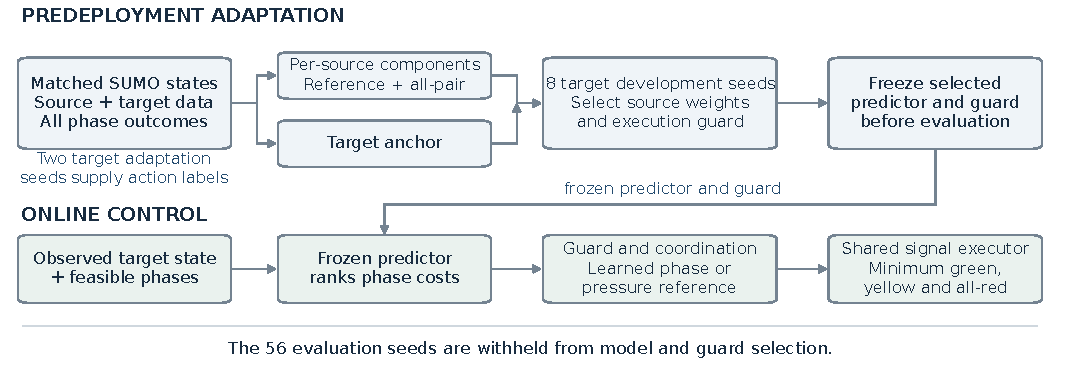
\includegraphics[width=\textwidth]{method_workflow.pdf}
\caption{Learning and deployment use different information. Matched simulator interventions provide source and target training outcomes. Two adaptation seeds supply target action labels; eight separate target development seeds select source weights and the execution guard. Deployment uses frozen predictors, the selected guard, sparse coordination, and current observations; evaluation outcomes are not used to select the controller.}
\label{fig:workflow}
\end{figure*}
